

\tikzset{every picture/.style={line width=0.75pt}} %set default line width to 0.75pt        

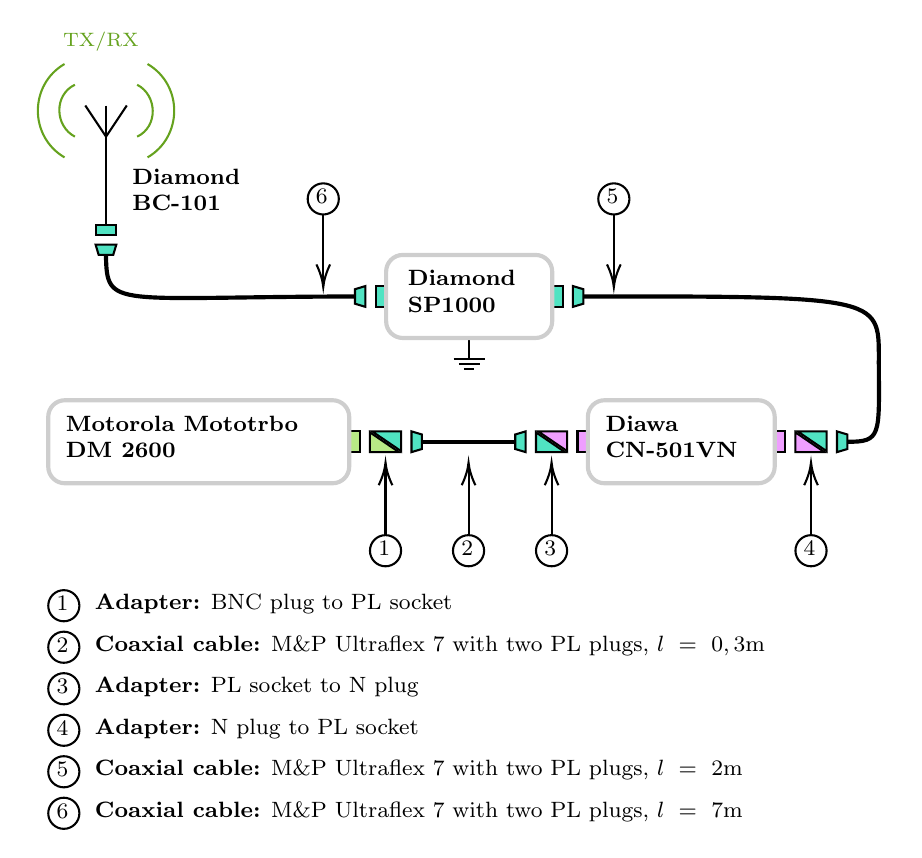
\begin{tikzpicture}[x=0.75pt,y=0.75pt,yscale=-1,xscale=1]
%uncomment if require: \path (0,479); %set diagram left start at 0, and has height of 479

%Straight Lines [id:da5218826641526857] 
\draw    (322.8,185) -- (322.8,195) ;
%Shape: Rectangle [id:dp3707976877259427] 
\draw  [fill={rgb, 255:red, 80; green, 227; blue, 194 }  ,fill opacity=1 ] (362.8,160) -- (367.8,160) -- (367.8,170) -- (362.8,170) -- cycle ;
%Shape: Rectangle [id:dp10664709959227037] 
\draw  [fill={rgb, 255:red, 80; green, 227; blue, 194 }  ,fill opacity=1 ] (277.8,160) -- (282.8,160) -- (282.8,170) -- (277.8,170) -- cycle ;
%Rounded Rect [id:dp527676076956175] 
\draw  [color={rgb, 255:red, 206; green, 206; blue, 206 }  ,draw opacity=1 ][line width=1.5]  (282.8,153) .. controls (282.8,148.58) and (286.38,145) .. (290.8,145) -- (354.8,145) .. controls (359.22,145) and (362.8,148.58) .. (362.8,153) -- (362.8,177) .. controls (362.8,181.42) and (359.22,185) .. (354.8,185) -- (290.8,185) .. controls (286.38,185) and (282.8,181.42) .. (282.8,177) -- cycle ;

%Straight Lines [id:da6289021026698145] 
\draw    (147.84,73) -- (147.84,133) ;
%Straight Lines [id:da47703805930667476] 
\draw    (137.84,73) -- (147.84,88) ;
%Straight Lines [id:da4218266835017126] 
\draw    (147.84,88) -- (157.84,73) ;
%Curve Lines [id:da5241031222048758] 
\draw [color={rgb, 255:red, 101; green, 162; blue, 30 }  ,draw opacity=1 ]   (162.84,63) .. controls (172.56,68) and (173.13,83.14) .. (162.84,88) ;
%Curve Lines [id:da3821737885384662] 
\draw [color={rgb, 255:red, 101; green, 162; blue, 30 }  ,draw opacity=1 ]   (167.84,53) .. controls (185.09,63.13) and (184.84,88.13) .. (167.84,98) ;

%Curve Lines [id:da3538255270661379] 
\draw [color={rgb, 255:red, 101; green, 162; blue, 30 }  ,draw opacity=1 ]   (132.84,88) .. controls (123.13,83) and (122.56,67.86) .. (132.84,63) ;
%Curve Lines [id:da889352578619292] 
\draw [color={rgb, 255:red, 101; green, 162; blue, 30 }  ,draw opacity=1 ]   (127.84,98) .. controls (110.59,87.88) and (110.84,62.87) .. (127.84,53) ;

%Shape: Rectangle [id:dp9150249297100126] 
\draw  [fill={rgb, 255:red, 80; green, 227; blue, 194 }  ,fill opacity=1 ] (142.84,130.5) -- (152.84,130.5) -- (152.84,135.5) -- (142.84,135.5) -- cycle ;
%Shape: Trapezoid [id:dp6261372647556653] 
\draw  [fill={rgb, 255:red, 80; green, 227; blue, 194 }  ,fill opacity=1 ][line width=0.75]  (152.8,140) -- (151.3,145) -- (144.3,145) -- (142.8,140) -- cycle ;
%Shape: Trapezoid [id:dp4286379946581531] 
\draw  [fill={rgb, 255:red, 80; green, 227; blue, 194 }  ,fill opacity=1 ][line width=0.75]  (272.8,170) -- (267.8,168.5) -- (267.8,161.5) -- (272.8,160) -- cycle ;
%Curve Lines [id:da8045163154695201] 
\draw [line width=1.5]    (147.8,145) .. controls (148.3,171.25) and (150.3,165.25) .. (267.8,165) ;
%Straight Lines [id:da19181563997268603] 
\draw    (315.3,195) -- (330.3,195) ;
%Straight Lines [id:da020619477423114985] 
\draw    (317.8,197.5) -- (327.8,197.5) ;
%Straight Lines [id:da9009961872255909] 
\draw    (320.3,200) -- (325.3,200) ;
%Shape: Rectangle [id:dp35598711466417887] 
\draw  [fill={rgb, 255:red, 239; green, 158; blue, 255 }  ,fill opacity=1 ] (470,230) -- (475,230) -- (475,240) -- (470,240) -- cycle ;
%Shape: Rectangle [id:dp4791882432942969] 
\draw  [fill={rgb, 255:red, 239; green, 158; blue, 255 }  ,fill opacity=1 ] (375,230) -- (380,230) -- (380,240) -- (375,240) -- cycle ;
%Shape: Rectangle [id:dp2776872187237942] 
\draw  [fill={rgb, 255:red, 184; green, 233; blue, 134 }  ,fill opacity=1 ] (265,230) -- (270,230) -- (270,240) -- (265,240) -- cycle ;
%Rounded Rect [id:dp5113702121898573] 
\draw  [color={rgb, 255:red, 206; green, 206; blue, 206 }  ,draw opacity=1 ][line width=1.5]  (120,223) .. controls (120,218.58) and (123.58,215) .. (128,215) -- (257,215) .. controls (261.42,215) and (265,218.58) .. (265,223) -- (265,247) .. controls (265,251.42) and (261.42,255) .. (257,255) -- (128,255) .. controls (123.58,255) and (120,251.42) .. (120,247) -- cycle ;

%Straight Lines [id:da5653713287945248] 
\draw [line width=1.5]    (300,235) -- (345,235) ;
%Shape: Trapezoid [id:dp6827000741886373] 
\draw  [fill={rgb, 255:red, 80; green, 227; blue, 194 }  ,fill opacity=1 ][line width=0.75]  (295,230) -- (300,231.5) -- (300,238.5) -- (295,240) -- cycle ;
%Shape: Trapezoid [id:dp5551727639514186] 
\draw  [fill={rgb, 255:red, 80; green, 227; blue, 194 }  ,fill opacity=1 ][line width=0.75]  (350,240) -- (345,238.5) -- (345,231.5) -- (350,230) -- cycle ;

%Shape: Right Triangle [id:dp6567087371846239] 
\draw  [fill={rgb, 255:red, 184; green, 233; blue, 134 }  ,fill opacity=1 ] (275,230.48) -- (288.98,240) -- (275,240) -- cycle ;
%Shape: Right Triangle [id:dp6439631638146213] 
\draw  [fill={rgb, 255:red, 80; green, 227; blue, 194 }  ,fill opacity=1 ] (290,239.52) -- (276.02,230) -- (290,230) -- cycle ;

%Shape: Right Triangle [id:dp7065836348516847] 
\draw  [fill={rgb, 255:red, 80; green, 227; blue, 194 }  ,fill opacity=1 ] (355,230.48) -- (368.98,240) -- (355,240) -- cycle ;
%Shape: Right Triangle [id:dp6791715198368578] 
\draw  [fill={rgb, 255:red, 239; green, 158; blue, 255 }  ,fill opacity=1 ] (370,239.52) -- (356.02,230) -- (370,230) -- cycle ;

%Rounded Rect [id:dp5242124209678602] 
\draw  [color={rgb, 255:red, 206; green, 206; blue, 206 }  ,draw opacity=1 ][line width=1.5]  (380,223) .. controls (380,218.58) and (383.58,215) .. (388,215) -- (462,215) .. controls (466.42,215) and (470,218.58) .. (470,223) -- (470,247) .. controls (470,251.42) and (466.42,255) .. (462,255) -- (388,255) .. controls (383.58,255) and (380,251.42) .. (380,247) -- cycle ;
%Shape: Right Triangle [id:dp9024696438630258] 
\draw  [fill={rgb, 255:red, 80; green, 227; blue, 194 }  ,fill opacity=1 ] (495,239.52) -- (481.02,230) -- (495,230) -- cycle ;
%Shape: Right Triangle [id:dp3027647623967811] 
\draw  [fill={rgb, 255:red, 239; green, 158; blue, 255 }  ,fill opacity=1 ] (480,230.48) -- (493.98,240) -- (480,240) -- cycle ;

%Curve Lines [id:da5556976336058517] 
\draw [line width=1.5]    (375.3,165) .. controls (526.33,164.83) and (520,165.25) .. (520.17,198.54) .. controls (520.34,231.82) and (521.33,235.17) .. (505,235) ;
%Shape: Trapezoid [id:dp7689909076073862] 
\draw  [fill={rgb, 255:red, 80; green, 227; blue, 194 }  ,fill opacity=1 ][line width=0.75]  (372.8,160) -- (377.8,161.5) -- (377.8,168.5) -- (372.8,170) -- cycle ;
%Shape: Trapezoid [id:dp5759023250736097] 
\draw  [fill={rgb, 255:red, 80; green, 227; blue, 194 }  ,fill opacity=1 ][line width=0.75]  (500,230) -- (505,231.5) -- (505,238.5) -- (500,240) -- cycle ;
%Straight Lines [id:da0668317935629783] 
\draw    (282.5,280) -- (282.5,247) ;
\draw [shift={(282.5,245)}, rotate = 450] [color={rgb, 255:red, 0; green, 0; blue, 0 }  ][line width=0.75]    (10.93,-3.29) .. controls (6.95,-1.4) and (3.31,-0.3) .. (0,0) .. controls (3.31,0.3) and (6.95,1.4) .. (10.93,3.29)   ;
%Shape: Circle [id:dp8618966688089644] 
\draw   (275,287.5) .. controls (275,283.36) and (278.36,280) .. (282.5,280) .. controls (286.64,280) and (290,283.36) .. (290,287.5) .. controls (290,291.64) and (286.64,295) .. (282.5,295) .. controls (278.36,295) and (275,291.64) .. (275,287.5) -- cycle ;


%Shape: Circle [id:dp06491171475414959] 
\draw   (315,287.5) .. controls (315,283.36) and (318.36,280) .. (322.5,280) .. controls (326.64,280) and (330,283.36) .. (330,287.5) .. controls (330,291.64) and (326.64,295) .. (322.5,295) .. controls (318.36,295) and (315,291.64) .. (315,287.5) -- cycle ;

%Straight Lines [id:da006440625484793738] 
\draw    (322.5,280) -- (322.5,247) ;
\draw [shift={(322.5,245)}, rotate = 450] [color={rgb, 255:red, 0; green, 0; blue, 0 }  ][line width=0.75]    (10.93,-3.29) .. controls (6.95,-1.4) and (3.31,-0.3) .. (0,0) .. controls (3.31,0.3) and (6.95,1.4) .. (10.93,3.29)   ;

%Shape: Circle [id:dp9167743181241499] 
\draw   (355,287.5) .. controls (355,283.36) and (358.36,280) .. (362.5,280) .. controls (366.64,280) and (370,283.36) .. (370,287.5) .. controls (370,291.64) and (366.64,295) .. (362.5,295) .. controls (358.36,295) and (355,291.64) .. (355,287.5) -- cycle ;

%Straight Lines [id:da48094261953448303] 
\draw    (362.5,280) -- (362.5,247) ;
\draw [shift={(362.5,245)}, rotate = 450] [color={rgb, 255:red, 0; green, 0; blue, 0 }  ][line width=0.75]    (10.93,-3.29) .. controls (6.95,-1.4) and (3.31,-0.3) .. (0,0) .. controls (3.31,0.3) and (6.95,1.4) .. (10.93,3.29)   ;

%Shape: Circle [id:dp1939511278206627] 
\draw   (480,287.5) .. controls (480,283.36) and (483.36,280) .. (487.5,280) .. controls (491.64,280) and (495,283.36) .. (495,287.5) .. controls (495,291.64) and (491.64,295) .. (487.5,295) .. controls (483.36,295) and (480,291.64) .. (480,287.5) -- cycle ;

%Straight Lines [id:da3351576985038338] 
\draw    (487.5,280) -- (487.5,247) ;
\draw [shift={(487.5,245)}, rotate = 450] [color={rgb, 255:red, 0; green, 0; blue, 0 }  ][line width=0.75]    (10.93,-3.29) .. controls (6.95,-1.4) and (3.31,-0.3) .. (0,0) .. controls (3.31,0.3) and (6.95,1.4) .. (10.93,3.29)   ;

%Shape: Circle [id:dp5129779571773962] 
\draw   (385,118) .. controls (385,113.86) and (388.36,110.5) .. (392.5,110.5) .. controls (396.64,110.5) and (400,113.86) .. (400,118) .. controls (400,122.14) and (396.64,125.5) .. (392.5,125.5) .. controls (388.36,125.5) and (385,122.14) .. (385,118) -- cycle ;

%Straight Lines [id:da6621400269321598] 
\draw    (392.5,158.5) -- (392.5,125.5) ;
\draw [shift={(392.5,160.5)}, rotate = 270] [color={rgb, 255:red, 0; green, 0; blue, 0 }  ][line width=0.75]    (10.93,-3.29) .. controls (6.95,-1.4) and (3.31,-0.3) .. (0,0) .. controls (3.31,0.3) and (6.95,1.4) .. (10.93,3.29)   ;

%Shape: Circle [id:dp7977203271441822] 
\draw   (245,118) .. controls (245,113.86) and (248.36,110.5) .. (252.5,110.5) .. controls (256.64,110.5) and (260,113.86) .. (260,118) .. controls (260,122.14) and (256.64,125.5) .. (252.5,125.5) .. controls (248.36,125.5) and (245,122.14) .. (245,118) -- cycle ;

%Straight Lines [id:da2162256591147207] 
\draw    (252.5,158.5) -- (252.5,125.5) ;
\draw [shift={(252.5,160.5)}, rotate = 270] [color={rgb, 255:red, 0; green, 0; blue, 0 }  ][line width=0.75]    (10.93,-3.29) .. controls (6.95,-1.4) and (3.31,-0.3) .. (0,0) .. controls (3.31,0.3) and (6.95,1.4) .. (10.93,3.29)   ;

%Shape: Circle [id:dp24834021243597504] 
\draw   (120,314) .. controls (120,309.86) and (123.36,306.5) .. (127.5,306.5) .. controls (131.64,306.5) and (135,309.86) .. (135,314) .. controls (135,318.14) and (131.64,321.5) .. (127.5,321.5) .. controls (123.36,321.5) and (120,318.14) .. (120,314) -- cycle ;

%Shape: Circle [id:dp7233992369838149] 
\draw   (120,334) .. controls (120,329.86) and (123.36,326.5) .. (127.5,326.5) .. controls (131.64,326.5) and (135,329.86) .. (135,334) .. controls (135,338.14) and (131.64,341.5) .. (127.5,341.5) .. controls (123.36,341.5) and (120,338.14) .. (120,334) -- cycle ;

%Shape: Circle [id:dp6313697664795326] 
\draw   (120,354) .. controls (120,349.86) and (123.36,346.5) .. (127.5,346.5) .. controls (131.64,346.5) and (135,349.86) .. (135,354) .. controls (135,358.14) and (131.64,361.5) .. (127.5,361.5) .. controls (123.36,361.5) and (120,358.14) .. (120,354) -- cycle ;

%Shape: Circle [id:dp03435814103609336] 
\draw   (120,374) .. controls (120,369.86) and (123.36,366.5) .. (127.5,366.5) .. controls (131.64,366.5) and (135,369.86) .. (135,374) .. controls (135,378.14) and (131.64,381.5) .. (127.5,381.5) .. controls (123.36,381.5) and (120,378.14) .. (120,374) -- cycle ;

%Shape: Circle [id:dp003390866078124999] 
\draw   (120,394) .. controls (120,389.86) and (123.36,386.5) .. (127.5,386.5) .. controls (131.64,386.5) and (135,389.86) .. (135,394) .. controls (135,398.14) and (131.64,401.5) .. (127.5,401.5) .. controls (123.36,401.5) and (120,398.14) .. (120,394) -- cycle ;

%Shape: Circle [id:dp7433181145978278] 
\draw   (120,414) .. controls (120,409.86) and (123.36,406.5) .. (127.5,406.5) .. controls (131.64,406.5) and (135,409.86) .. (135,414) .. controls (135,418.14) and (131.64,421.5) .. (127.5,421.5) .. controls (123.36,421.5) and (120,418.14) .. (120,414) -- cycle ;



% Text Node
\draw (159,102) node [anchor=north west][inner sep=0.75pt]  [font=\footnotesize] [align=left] {\textbf{Diamond }\\\textbf{BC-101}};
% Text Node
\draw (127,221) node [anchor=north west][inner sep=0.75pt]  [font=\footnotesize] [align=left] {\textbf{Motorola Mototrbo}\\\textbf{DM 2600}};
% Text Node
\draw (387,221) node [anchor=north west][inner sep=0.75pt]  [font=\footnotesize] [align=left] {\textbf{Diawa}\\\textbf{CN-501VN}};
% Text Node
\draw (291.8,151) node [anchor=north west][inner sep=0.75pt]  [font=\footnotesize] [align=left] {\textbf{Diamond}\\\textbf{SP1000}};
% Text Node
\draw (125.69,36) node [anchor=north west][inner sep=0.75pt]  [font=\scriptsize,color={rgb, 255:red, 101; green, 162; blue, 30 }  ,opacity=1 ] [align=left] {TX/RX};
% Text Node
\draw (277.5,281.5) node [anchor=north west][inner sep=0.75pt]  [font=\footnotesize] [align=left] {1};
% Text Node
\draw (317.5,281.5) node [anchor=north west][inner sep=0.75pt]  [font=\footnotesize] [align=left] {2};
% Text Node
\draw (357.5,281.5) node [anchor=north west][inner sep=0.75pt]  [font=\footnotesize] [align=left] {3};
% Text Node
\draw (482.5,281.5) node [anchor=north west][inner sep=0.75pt]  [font=\footnotesize] [align=left] {4};
% Text Node
\draw (387.5,112) node [anchor=north west][inner sep=0.75pt]  [font=\footnotesize] [align=left] {5};
% Text Node
\draw (247.5,112) node [anchor=north west][inner sep=0.75pt]  [font=\footnotesize] [align=left] {6};
% Text Node
\draw (122.5,308) node [anchor=north west][inner sep=0.75pt]  [font=\footnotesize] [align=left] {1};
% Text Node
\draw (122.5,328) node [anchor=north west][inner sep=0.75pt]  [font=\footnotesize] [align=left] {2};
% Text Node
\draw (122.5,348) node [anchor=north west][inner sep=0.75pt]  [font=\footnotesize] [align=left] {3};
% Text Node
\draw (122.5,368) node [anchor=north west][inner sep=0.75pt]  [font=\footnotesize] [align=left] {4};
% Text Node
\draw (122.5,388) node [anchor=north west][inner sep=0.75pt]  [font=\footnotesize] [align=left] {5};
% Text Node
\draw (122.5,408) node [anchor=north west][inner sep=0.75pt]  [font=\footnotesize] [align=left] {6};
% Text Node
\draw (141,307) node [anchor=north west][inner sep=0.75pt]  [font=\footnotesize] [align=left] {\textbf{Adapter:} BNC plug to PL socket};
% Text Node
\draw (141,327) node [anchor=north west][inner sep=0.75pt]  [font=\footnotesize] [align=left] {\textbf{Coaxial cable:} M\&P Ultraflex 7 with two PL plugs, $\displaystyle l\ =\ 0,3\mathrm{m}$};
% Text Node
\draw (141,347) node [anchor=north west][inner sep=0.75pt]  [font=\footnotesize] [align=left] {\textbf{Adapter:} PL socket to N plug};
% Text Node
\draw (141,367) node [anchor=north west][inner sep=0.75pt]  [font=\footnotesize] [align=left] {\textbf{Adapter:} N plug to PL socket};
% Text Node
\draw (141,387) node [anchor=north west][inner sep=0.75pt]  [font=\footnotesize] [align=left] {\textbf{Coaxial cable:} M\&P Ultraflex 7 with two PL plugs, $\displaystyle l\ =\ 2\mathrm{m}$};
% Text Node
\draw (141,407) node [anchor=north west][inner sep=0.75pt]  [font=\footnotesize] [align=left] {\textbf{Coaxial cable:} M\&P Ultraflex 7 with two PL plugs, $\displaystyle l\ =\ 7\mathrm{m}$};


\end{tikzpicture}
